%!TEX root = ../../thesis.tex

The Standard Model of particle physics (SM) is a quantum field theory describing
the kinematics and interactions of sub-atomic particles. The dynamics of such a 
theory are determined by the symmetries respected by the Lagrangian density.
The SM is invariant under local transformations of the \SMgroup gauge group,
resulting in the strong, weak and electromagnetic forces of nature and determining
the particle content of the theory. Additionally, invariance under global 
transformations of the Poincaré group ensures the theory is identical in all 
inertial frames of reference, as asserted by special relativity.

Each gauge theory of the SM describes the dynamics of a force of nature, which 
is mediated by a number of gauge bosons and couples to a conserved current, in 
accordance with Noether's theorem. Quantum chromodynamics (QCD) describes the strong 
interaction, is mediated by eight gluons and couples to colour charge. Quantum 
electrodynamics (QED) describes the electromagnetic interaction, is mediated by the 
photon and couples to electric charge. The weak interaction is mediated by the massive 
\PWpm and \PZzero bosons and is understood within the context of electroweak theory (EW),
a unification of the electromagnetic and weak interactions. A quantum field theory of
gravity is not included in the SM. It is important to note that the gauge groups of the
strong and weak interactions are non-abelian. Physically, this means that the
gauge bosons are themselves charged and therefore experience self-interactions.

\begin{figure}
	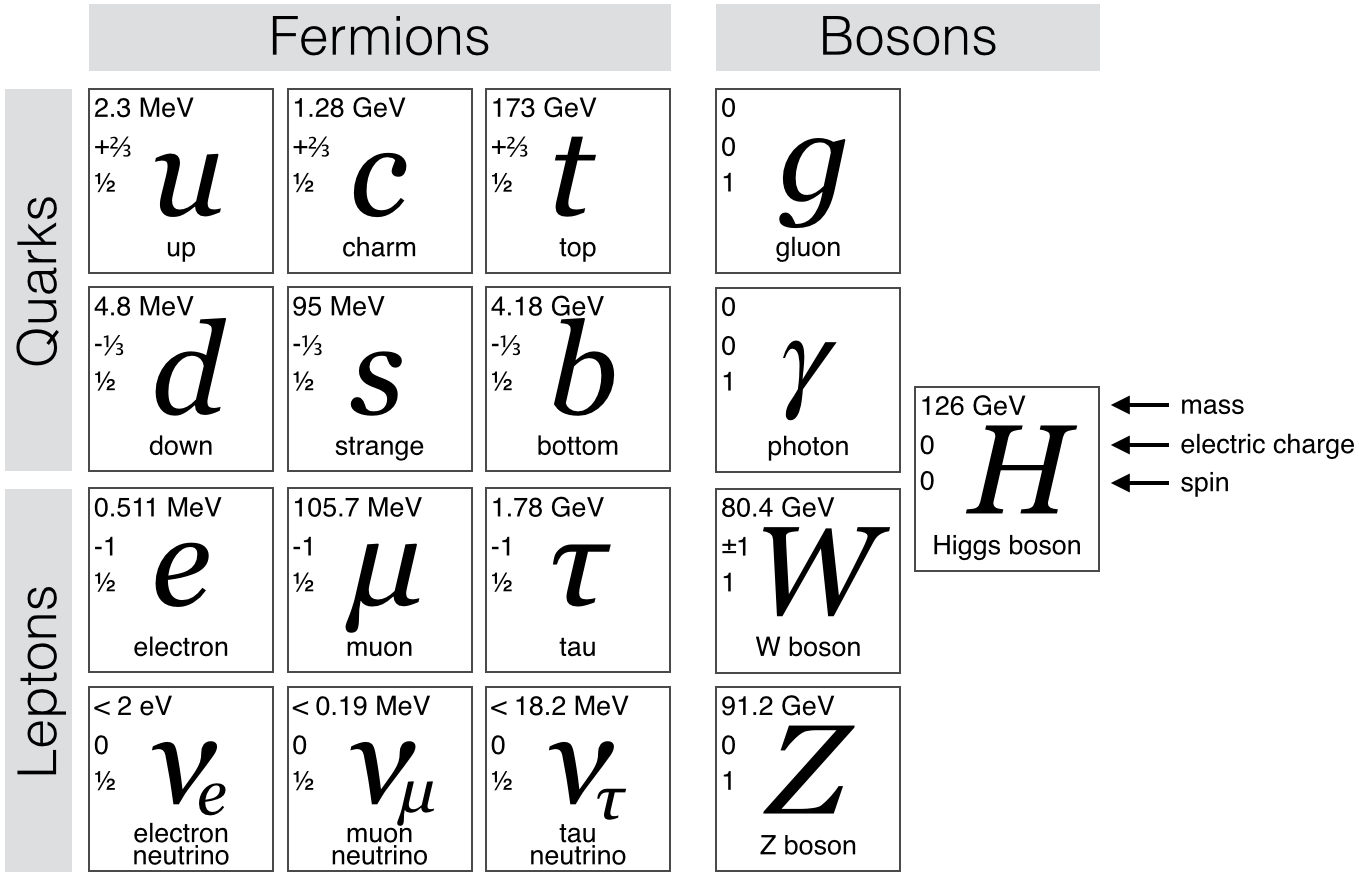
\includegraphics[width=\largefigwidth]{tex/motivation/sm_particles}
	\caption{The particle content of the Standard Model. Mass data from \cite{PDG}.}
	\label{fig:sm_particles}
\end{figure}

The elementary particles of the SM are summarised in \Figure~\ref{fig:sm_particles}.
They are naturally separated into bosons (integer spin) and fermions (half-integer spin).
In addition to the gauge bosons previously introduced, the Higgs boson is a by-product
of electroweak symmetry breaking (described in \Section~\ref{sec:ewsb}) and its
couplings are proportional to mass. The fermions are categorised according to the
interactions they experience, or equivalently the charges they posses: quarks
(strong, electromagnetic, weak), charged leptons (electromagnetic, weak) and neutrinos 
(weak). Most particles also have an associated antiparticle with identical mass
but inverted internal quantum numbers.
